\documentclass[tikz,border=6pt]{standalone}
\usepackage[T1]{fontenc}
\usepackage{lmodern}
\usepackage{amsmath,amssymb}
\usepackage{tikz}
\usetikzlibrary{positioning,arrows.meta,shapes.geometric,calc}

% Matched to style/tikz_style.tex; kept local so the asset is reproducible.
\tikzset{
  bdc arrow/.style={-{Stealth[length=2.2mm,width=1.6mm]},line width=0.8pt,black},
  bdc state/.style={draw=black,line width=0.8pt,rounded corners=2pt,
    minimum width=7.5mm,minimum height=7.5mm,inner sep=1pt,font=\small},
  bdc absorbing/.style={bdc state,fill=gray!10,line width=1.0pt},
  bdc catastrophe/.style={draw=black,line width=1.0pt,ellipse,
    minimum width=9mm,minimum height=7.5mm,inner sep=1pt,font=\small,fill=gray!8},
  bdc ratelabel/.style={font=\small,inner sep=1pt,fill=white,
    fill opacity=0.88,text opacity=1},
  bdc annotation/.style={font=\small\itshape,text=black!70}
}

\begin{document}
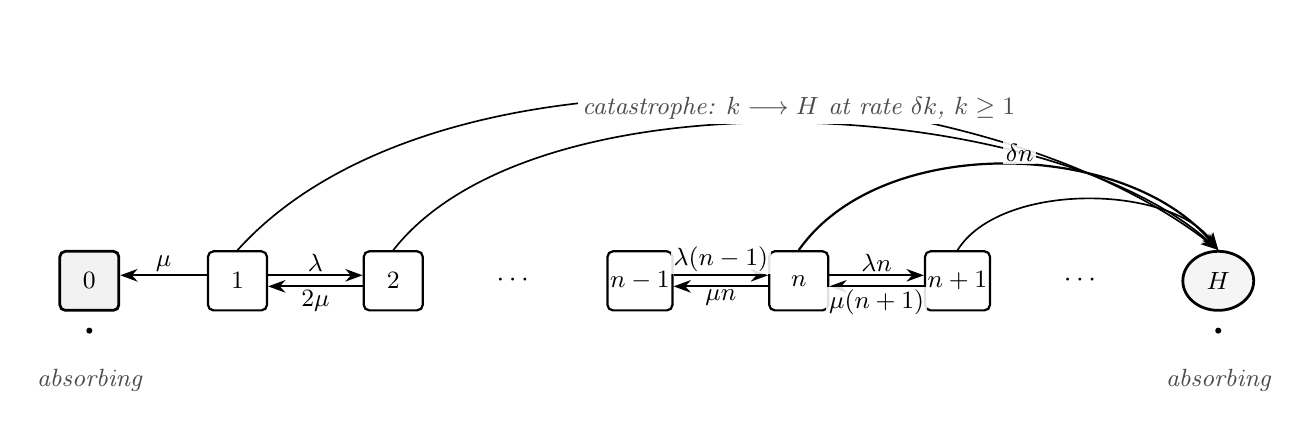
\begin{tikzpicture}[font=\small]
  \node[bdc absorbing] (zero) {$0$};
  \node[bdc state,right=11mm of zero] (one) {$1$};
  \node[bdc state,right=12mm of one] (two) {$2$};
  \node[right=8mm of two,font=\normalsize] (dotsa) {$\cdots$};
  \node[bdc state,right=8mm of dotsa] (nm) {$n-1$};
  \node[bdc state,right=12mm of nm] (n) {$n$};
  \node[bdc state,right=12mm of n] (np) {$n+1$};
  \node[right=8mm of np,font=\normalsize] (dotsb) {$\cdots$};
  \node[bdc catastrophe,right=9mm of dotsb] (H) {$H$};

  % Representative low-state transitions; zero has no outgoing arrow.
  \draw[bdc arrow] ([yshift=2pt]one.west) --
    node[bdc ratelabel,above] {$\mu$} ([yshift=2pt]zero.east);
  \draw[bdc arrow] ([yshift=2pt]one.east) --
    node[bdc ratelabel,above] {$\lambda$} ([yshift=2pt]two.west);
  \draw[bdc arrow] ([yshift=-2pt]two.west) --
    node[bdc ratelabel,below] {$2\mu$} ([yshift=-2pt]one.east);

  % Generic local transitions show the exact state-dependent rates.
  \draw[bdc arrow] ([yshift=2pt]nm.east) --
    node[bdc ratelabel,above] {$\lambda(n-1)$} ([yshift=2pt]n.west);
  \draw[bdc arrow] ([yshift=-2pt]n.west) --
    node[bdc ratelabel,below] {$\mu n$} ([yshift=-2pt]nm.east);
  \draw[bdc arrow] ([yshift=2pt]n.east) --
    node[bdc ratelabel,above] {$\lambda n$} ([yshift=2pt]np.west);
  \draw[bdc arrow] ([yshift=-2pt]np.west) --
    node[bdc ratelabel,below] {$\mu(n+1)$} ([yshift=-2pt]n.east);

  % Catastrophe transitions.  The labelled generic arrow states the rule;
  % the thinner outer arrows make clear that it applies to every k >= 1.
  \draw[bdc arrow,line width=0.6pt] (one.north) to[out=48,in=142,looseness=0.78] (H.north);
  \draw[bdc arrow,line width=0.6pt] (two.north) to[out=52,in=138,looseness=0.72] (H.north);
  \draw[bdc arrow] (n.north) to[out=55,in=130,looseness=0.88]
    node[bdc ratelabel,pos=0.53,above] {$\delta n$} (H.north);
  \draw[bdc arrow,line width=0.6pt] (np.north) to[out=58,in=126,looseness=0.8] (H.north);
  \node[bdc annotation,fill=white,inner sep=1.5pt,above=16mm of n] (catrule)
    {catastrophe: $k\longrightarrow H$ at rate $\delta k$, $k\geq1$};

  \node[bdc annotation,below=6mm of zero] {absorbing};
  \node[bdc annotation,below=6mm of H] {absorbing};
  \fill (zero.south) ++(0,-2.4mm) circle[radius=1.1pt];
  \fill (H.south) ++(0,-2.4mm) circle[radius=1.1pt];
\end{tikzpicture}
\end{document}
